\documentclass[uplatex,a4paper,12pt]{jsarticle}

%% フォント
%\usepackage{newtxtext,newtxmath}
%% 図、文字色
\usepackage[dvipdfmx]{graphicx,xcolor}
%% ハイパーリンク
\usepackage[dvipdfmx]{hyperref}
%% しおりの日本語
\usepackage{pxjahyper}
%% しおりに節番号を含める、リンクの枠を出力しない
\hypersetup{
  bookmarksnumbered=true,
  hidelinks=true,
  colorlinks=false,
}
%% 特殊記号
\usepackage{textcomp}
%% URL
\usepackage{url}
%% 表
%\usepackage{multirow}
%% 参照漏れチェック(デバッグ用)
%\usepackage{refcheck}


\usepackage{subcaption}

% 図と表の表記
\renewcommand{\figurename}{Fig.}
\renewcommand{\tablename}{Table.}
\newcommand{\figref}[1]{\figurename~\ref{#1}}
\newcommand{\tabref}[1]{\tablename~\ref{#1}}

% キャプションとページ番号をゴシック体に
\renewcommand{\kanjifamilydefault}{\gtdefault}
\usepackage{caption}
\usepackage{fancyhdr,lastpage}
\fancypagestyle{foot}
{
  \lhead{}
  \chead{}
  \rhead{}
  \cfoot{{\sf \thepage{}/{}\pageref{LastPage}}}
  \renewcommand{\headrulewidth}{0.0pt}
}

\usepackage[top=30truemm,bottom=30truemm,left=30truemm,right=30truemm]{geometry}
\usepackage{here}
\usepackage{fancyhdr}
\usepackage{lastpage}
\fancypagestyle{mypagestyle}{%
\lhead{}%ヘッダ左を空に
\rhead{}%ヘッダ右を空に
\cfoot{\thepage/\pageref{LastPage}}%フッタ中央に"今のページ数/総ページ数"を設定
\renewcommand{\headrulewidth}{0.0pt}%ヘッダの線を消す
}
\pagestyle{mypagestyle}
\begin{document}

% http://www.latex-cmd.com/style/style.html
% \gt % ゴシック体
% \sf % サンセリフ体
\gtfamily\sffamily

\makeatletter
\renewcommand{\section}{\@startsection{section}{1}{\z@}{1.5\Cvs \@plus.5\Cvs \@minus.2\Cvs}{.5\Cvs \@plus.3\Cvs}{\reset@font\bfseries\gtfamily\sffamily}}
\renewcommand{\subsection}{\@startsection{subsection}{1}{\z@}{1.5\Cvs \@plus.5\Cvs \@minus.2\Cvs}{.5\Cvs \@plus.3\Cvs}{\reset@font\bfseries\gtfamily\sffamily}}
\makeatother
\captionsetup[figure]{font=sf}
\pagestyle{foot}

\pagenumbering{arabic}
\setcounter{page}{1}

% タイトルとサブタイトル(ad-hoc)
%% maketitleでタイトルを入れたければ、プリアンブルを調整して同じ様に表示されるようにしてください。
\begin{center}
\fontsize{14pt}{0pt}\selectfont
ぬいぐるみ専用の組み込みAIモジュールの開発\\
- あらゆるぬいぐるみに さらなる命を吹き込む - 
\end{center}
    

\section{背景}
% 近年、新型コロナウイルスの流行を受けた生活様式の変化もあって、一人暮らしの学生の孤独が問題となっている。
% 日々の癒やしを求めてペットの飼育が一時的なブームとなったが、一人暮らしでは世話や費用の面からペットを飼育することは難しい。
% ペットに代わる存在として、管理の楽な愛玩用ロボットもいくつか市販されている。
% しかし、それらは工業製品としての性格が強く同じ製品ならばどれも同じ外観であるため、対象に愛着を感じる上で重要な目の前の相手がこの世に一人しかいないというオンリーワンの要素に乏しい一面がある。
% ところで、より広く普及している愛玩対象として、ぬいぐるみがある。
% ぬいぐるみは手間がかからないにもかかわらず、柔らかい手触りで安心感を与えてくれる。
% さらに、犬や熊など様々な種類のものが市販されているため、人の好みに寄り添うことができる。
% したがって、もしぬいぐるみをロボット化できれば、ユーザの好みに寄り添った愛玩対象を生み出せると考えられる。
% しかし、様々な種類のぬいぐるみそれぞれについて独立した過程でロボット化することは、開発コストの観点から現実的でない。
情報化が進んだ現代においても、一人暮らしなどで人が孤独を感じることは多い。
心の癒やしとしてペットの飼育が考えられるが、一人暮らしで世話を行うことは難しい。
そういった背景も踏まえてか、近年では愛玩用ロボットなども販売され始めている。
しかし、これらは工業製品であるがゆえに同じ製品ならば見た目はどれも同じであり、オンリーワンの要素に乏しい。

そこで本プロジェクトでは、人が適度な距離感で触れ合え、かつ多様な種類が存在するぬいぐるみに注目する。
そして、ぬいぐるみをロボット化することで現代の生活に即した心の癒やしを生み出そうと考えた。
しかし、ユーザの好みに応えるべく多くの種類が存在するぬいぐるみをすべてロボット化することは開発コストの観点から難しい。


\section{目的}
そこで本プロジェクトのでは、ぬいぐるみのロボット化に特化した組み込みAIモジュールを開発し、ぬいぐるみの骨格の規格化を目指す。
具体的には、多くの種類のぬいぐるみを効率的にロボット化するために、ぬいぐるみロボットを機械的・電気的要素を含む共通の内部骨格と換装可能なぬいぐるみ部分に分割する。
これにより、ユーザはロボットの骨格と好きな種類のぬいぐるみを組み合わせることで、たとえぬいぐるみが犬型であっても熊型であっても、同じ骨格を組み込むことで好みの見た目のぬいぐるみロボットを簡単に手にするとが可能となる(\figref{fig:mohutics:concept_embed})。
本プロジェクトではロボットの共通化された内部骨格と、それに対応する複数のぬいぐるみを実際に製作し、毛皮の換装可能なぬいぐるみロボットシステムの実現を目指す。

\begin{figure}[htbp]
  \centering
  \begin{minipage}[c]{0.48\linewidth}
    \centering
    \includegraphics[keepaspectratio,width=4cm,clip]{images/mohutics/concept_dog.png}
    \subcaption{犬のぬいぐるみへの埋め込み}
    \label{fig:mohutics:concept_dog}
  \end{minipage}
  \begin{minipage}[c]{0.48\linewidth}
    \centering
    \includegraphics[keepaspectratio,width=4cm,clip]{images/mohutics/concept_bear.png}
    \subcaption{熊のぬいぐるみへの埋め込み}
    \label{fig:mohutics:concept_bear}
  \end{minipage}
  \caption{共通骨格を異なるぬいぐるみに埋め込む概念図}
  \label{fig:mohutics:concept_embed}
\end{figure}

\section{開発の内容}
\subsection{ぬいぐるみロボットの内部骨格}
本システムでは共通の内部骨格として、5関節を持つ直径約8cm、全長約40cmのシリアルリンクロボットを製作した(\figref{fig:mohucore:serial_link}・\figref{fig:mohucore:skeleton})。
ロボットとしては簡素な構造であるが、本物の動物のように四肢を正確に動かすのではなく、様々なぬいぐるみに対応するぬいぐるみロボットとして必要十分な機能を備えることに重点を置いた。
この骨格にはESP32マイクロコントローラやサーボモータ、姿勢センサ、感圧センサ等が取り付けられている。
そして、Wi-Fiを経由してインターネット上からプログラムを取得し、ロボットが動作する。
なお、感圧センサを12個使用したため、メインCPUとは別にPICマイコンを使用してアナログ入力端子の不足を補うなどしている。

\begin{figure}[htbp]
  \centering
  \begin{minipage}[c]{0.48\linewidth}
    \centering
    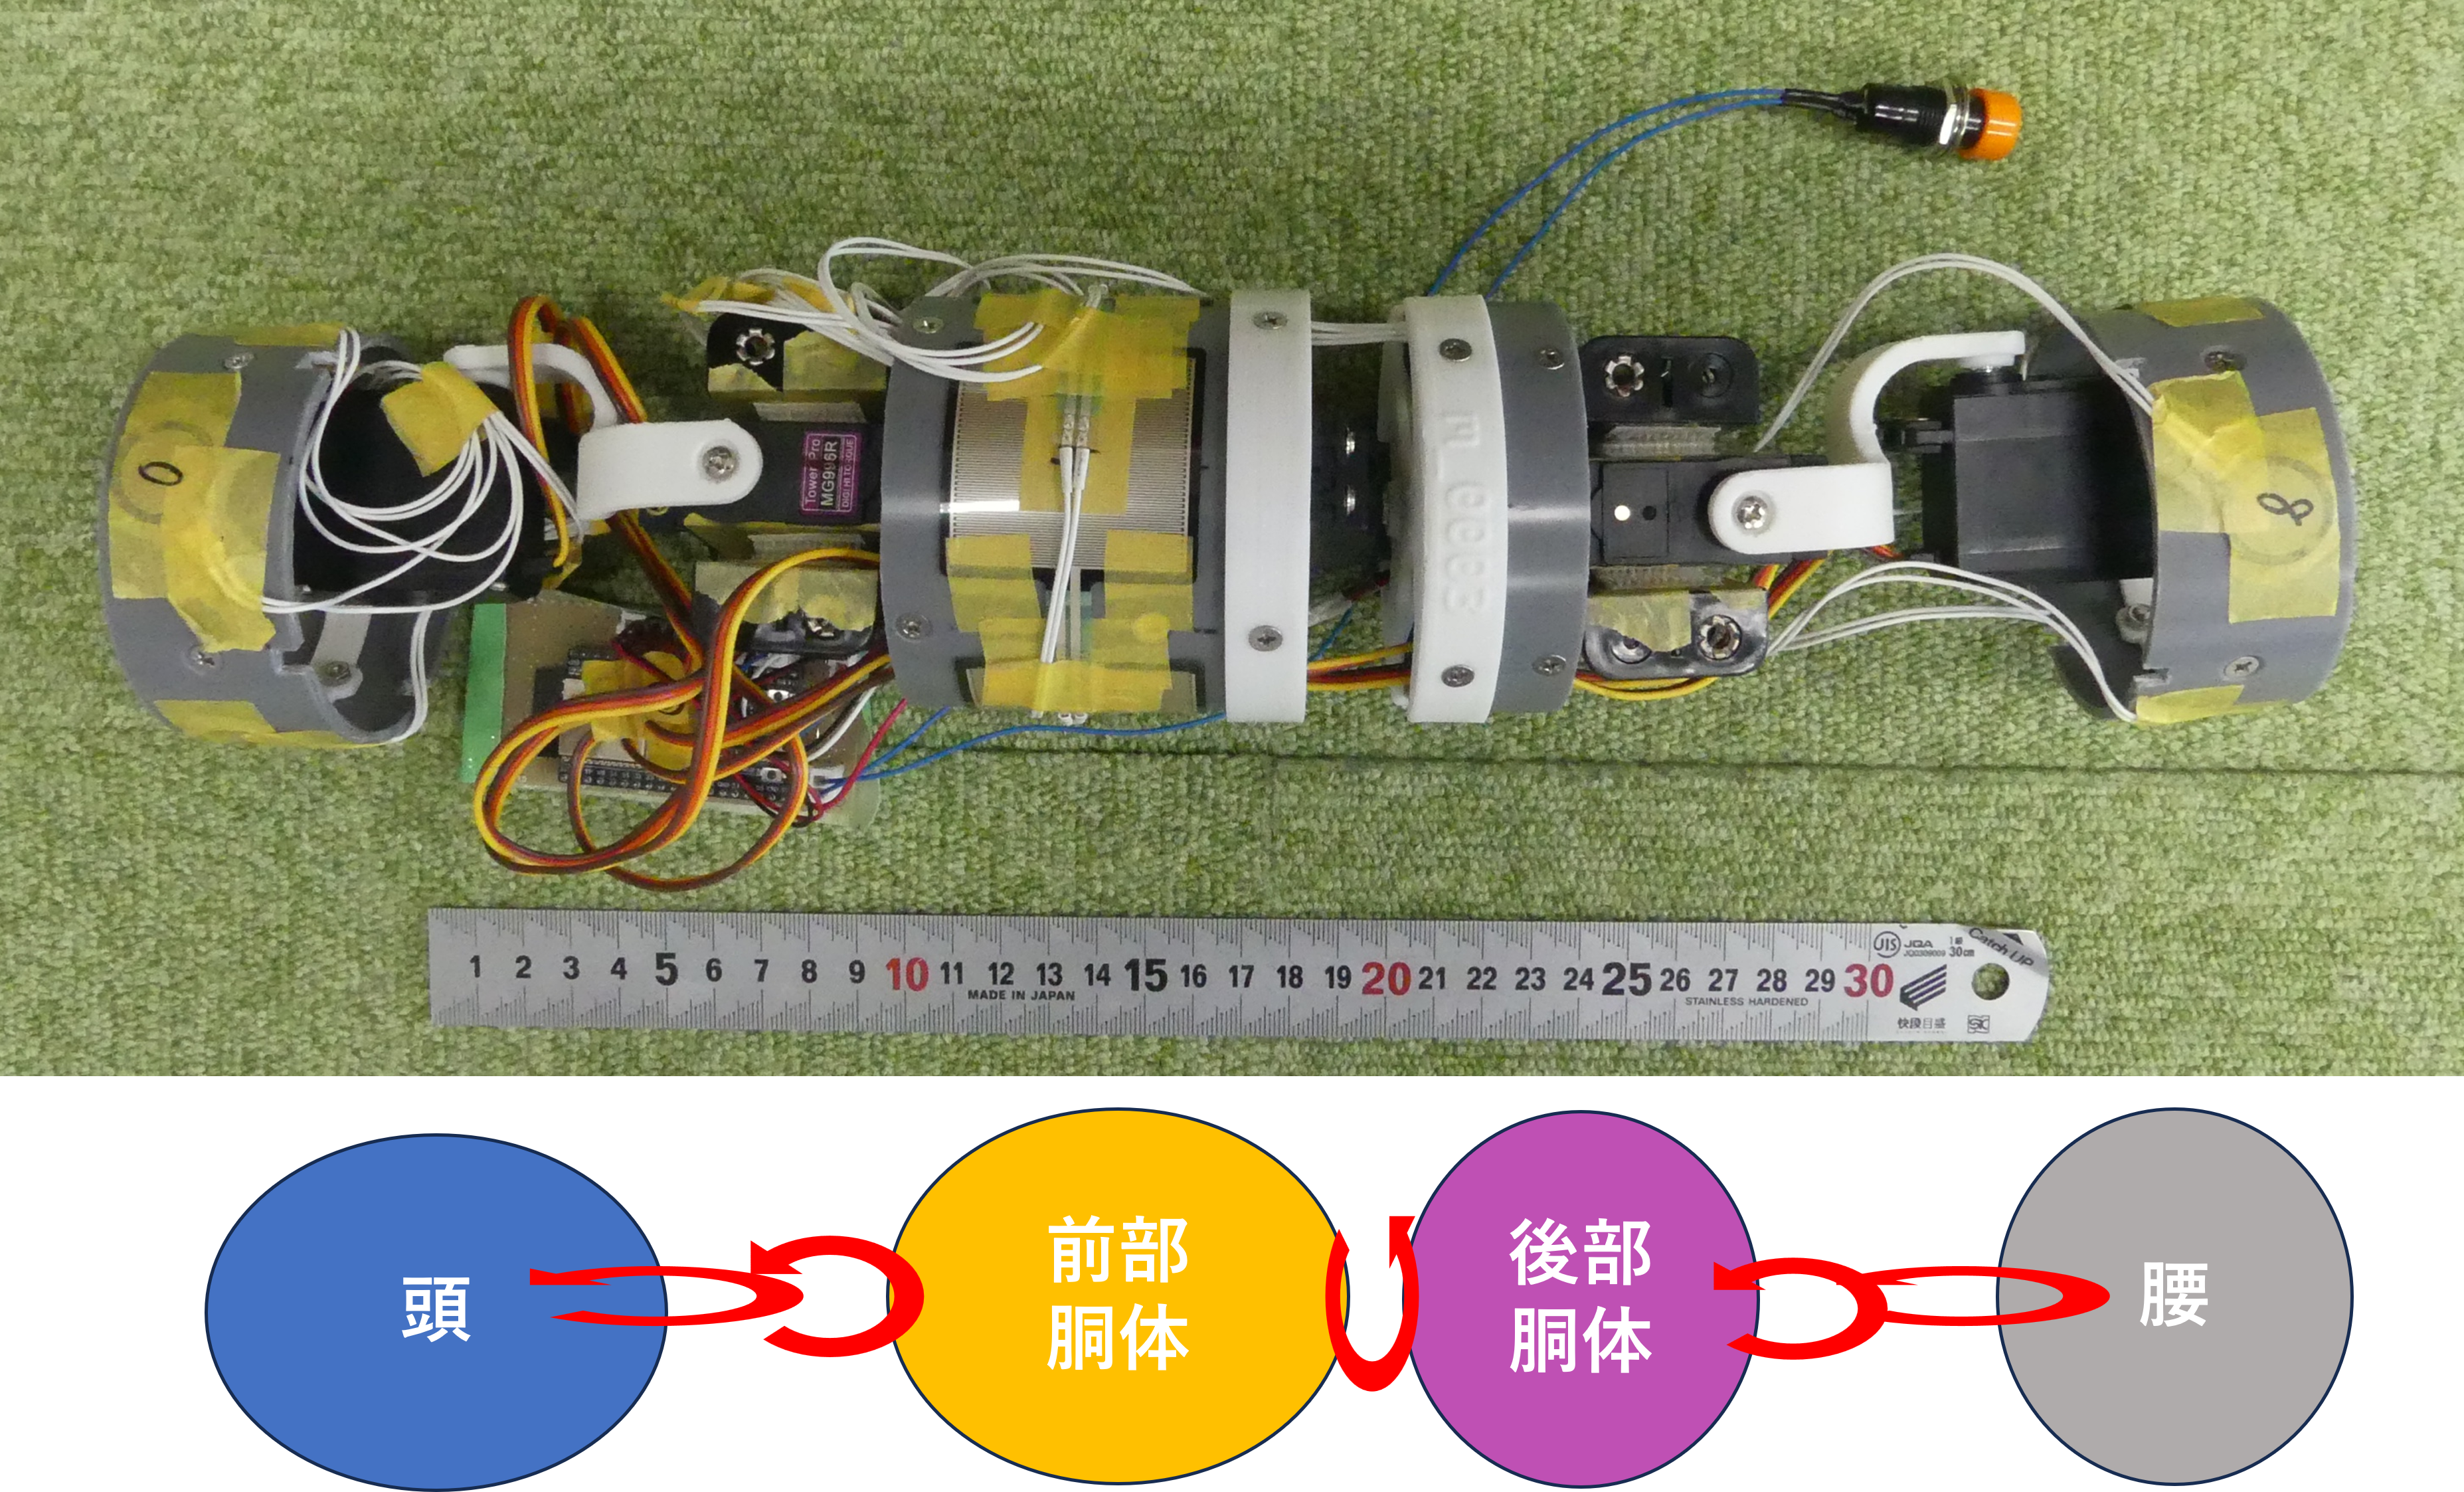
\includegraphics[keepaspectratio,width=6cm,clip]{images/mohucore/5motors.png}
    \subcaption{シリアルリンクの模式図}
  \end{minipage}
  \begin{minipage}[c]{0.48\linewidth}
    \centering
    \includegraphics[keepaspectratio,width=6cm,clip]{images/mohucore/rot_arrangement.png}
    \subcaption{回転軸の配置}
  \end{minipage}
  \caption{内部骨格のシリアルリンクの構造と回転軸の配置}
  \label{fig:mohucore:serial_link}
\end{figure}



\begin{figure}[htbp]
  \centering
  \includegraphics[width=8cm]{images/mohucore/skeleton.jpg}
  \caption{内部骨格の外観}
  \label{fig:mohucore:skeleton}
\end{figure}


\subsection{ぬいぐるみロボットに対応するぬいぐるみ}
ぬいぐるみの骨格に取り付けられるぬいぐるみとして、本プロジェクトでは完全新規設計のものと市販品を改造したものを製作した。
本システムの骨格の性能を十分に活かすにはぬいぐるみも骨格に合わせて設計することが望ましい。
一方で世の中にはすでに多くのぬいぐるみが出回っており、自分の好きな既製品のぬいぐるみに少し手を加えてロボットにしたいユーザも一定数いると考えられるため、市販品を改造したものも用意した。

完全新規設計のぬいぐるみについては、まず3DCGソフトウェアで犬型のぬいぐるみをモデリングした(\figref{fig:mohukawa:blender})。
そして、UV展開機能を用いて展開図を出力し、それに合わせて型紙を作成し生地を裁断・縫製するなどして(\figref{fig:mohukawa:dog})のような犬型のぬいぐるみを製作した。

\begin{figure}[htbp]
  \centering
  \begin{minipage}[c]{0.56\linewidth}
    \centering
    \includegraphics[keepaspectratio,width=8cm,clip]{images/mohukawa/blender_01.png}
    \subcaption{三面図}
    \label{fig:mohukawa:blender_01}
  \end{minipage}
  \begin{minipage}[c]{0.40\linewidth}
    \centering
    \includegraphics[keepaspectratio,width=6cm,clip]{images/mohukawa/dog_sensor.png}
    \subcaption{骨格とぬいぐるみの毛皮の配置図}
    \label{fig:mohukawa:blender_02}
  \end{minipage}
  \caption{3DCGソフトウェアによる犬のぬいぐるみのモデリング}
  \label{fig:mohukawa:blender}
\end{figure}

\begin{figure}[htbp]
  \centering
  \begin{minipage}[c]{0.64\linewidth}
    \centering
    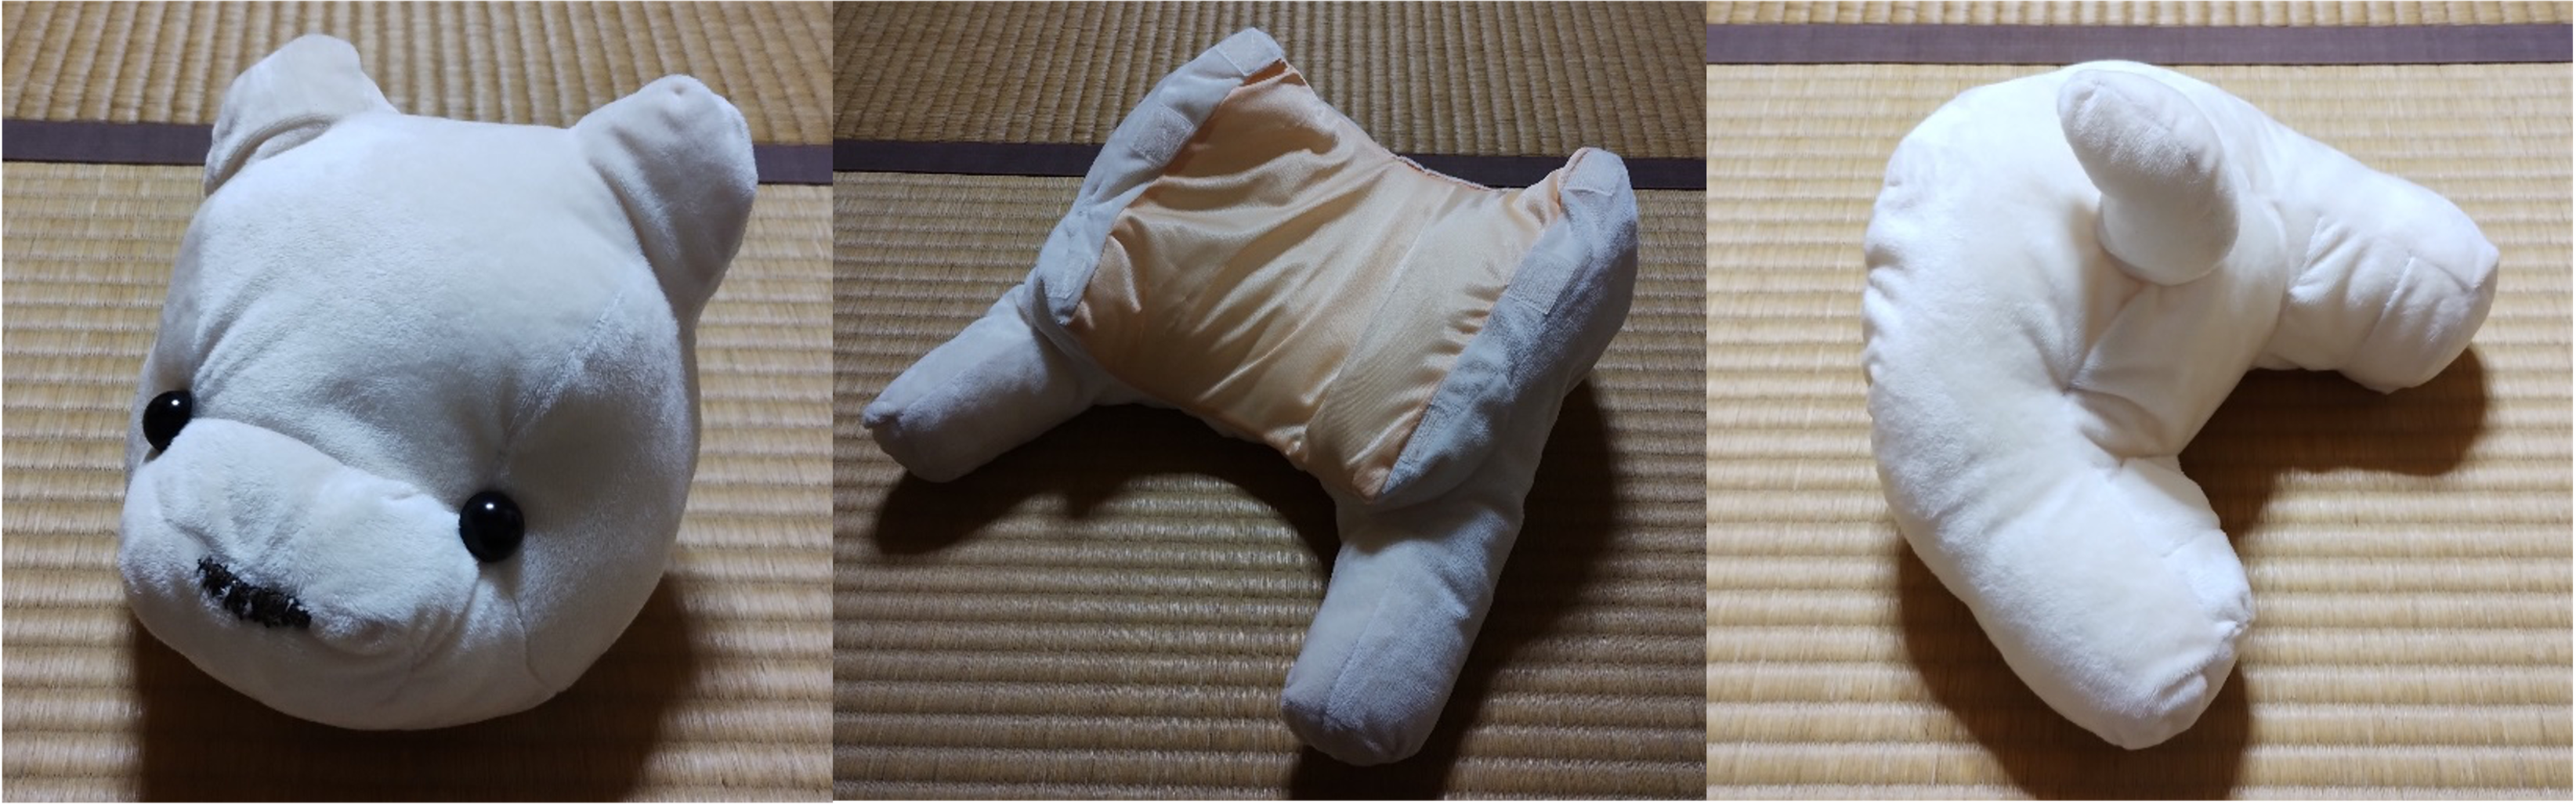
\includegraphics[keepaspectratio,width=8cm,clip]{images/mohukawa/dog_parts.png}
    \subcaption{犬型のぬいぐるみの各パーツ(頭・胴・腰)}
  \end{minipage}
  \begin{minipage}[c]{0.32\linewidth}
    \centering
    \includegraphics[keepaspectratio,width=4cm,clip]{images/mohukawa/dog.jpg}
    \subcaption{犬型のぬいぐるみ}
  \end{minipage}
  \caption{完全新規設計のぬいぐるみ}
  \label{fig:mohukawa:dog}
\end{figure}

さらに、市販品を改造したぬいぐるみについては、一度ぬいぐるみを切り開いたのちにぬいぐるみ内部に空洞を作るように布をあてがい、再度綿を詰めるなどの加工を施した。
そして、本システムに対応する人型・アナゴ型・パンダ型のぬいぐるみを用意した(\figref{fig:mohukawa:funio_anago_panda})。

\begin{figure}[htbp]
  \centering
  \begin{minipage}[c]{0.32\linewidth}
    \centering
    \includegraphics[keepaspectratio,width=4cm,clip]{images/mohukawa/funio.jpg}
    \subcaption{人型のぬいぐるみ}
  \end{minipage}
  \begin{minipage}[c]{0.32\linewidth}
    \centering
    \includegraphics[keepaspectratio,width=4cm,clip]{images/mohukawa/anago.jpg}
    \subcaption{アナゴ型のぬいぐるみ}
  \end{minipage}
  \begin{minipage}[c]{0.32\linewidth}
    \centering
    \includegraphics[keepaspectratio,width=4cm,clip]{images/mohukawa/panda.jpg}
    \subcaption{パンダ型のぬいぐるみ}
  \end{minipage}
  \caption{市販品を改造して製作されたMohuKawa}
  \label{fig:mohukawa:funio_anago_panda}
\end{figure}

製作した骨格とぬいぐるみは工具を使わずに手で簡単に組み立てられる。
いずれのぬいぐるみについても、およそ1分30秒でぬいぐるみを骨格に取り付けることが可能であった(\figref{fig:mohutics:embed_dog}・\figref{fig:mohutics:embed_funio})。

\begin{figure}[htbp]
  \centering
  \begin{minipage}[c]{\linewidth}
    \centering
    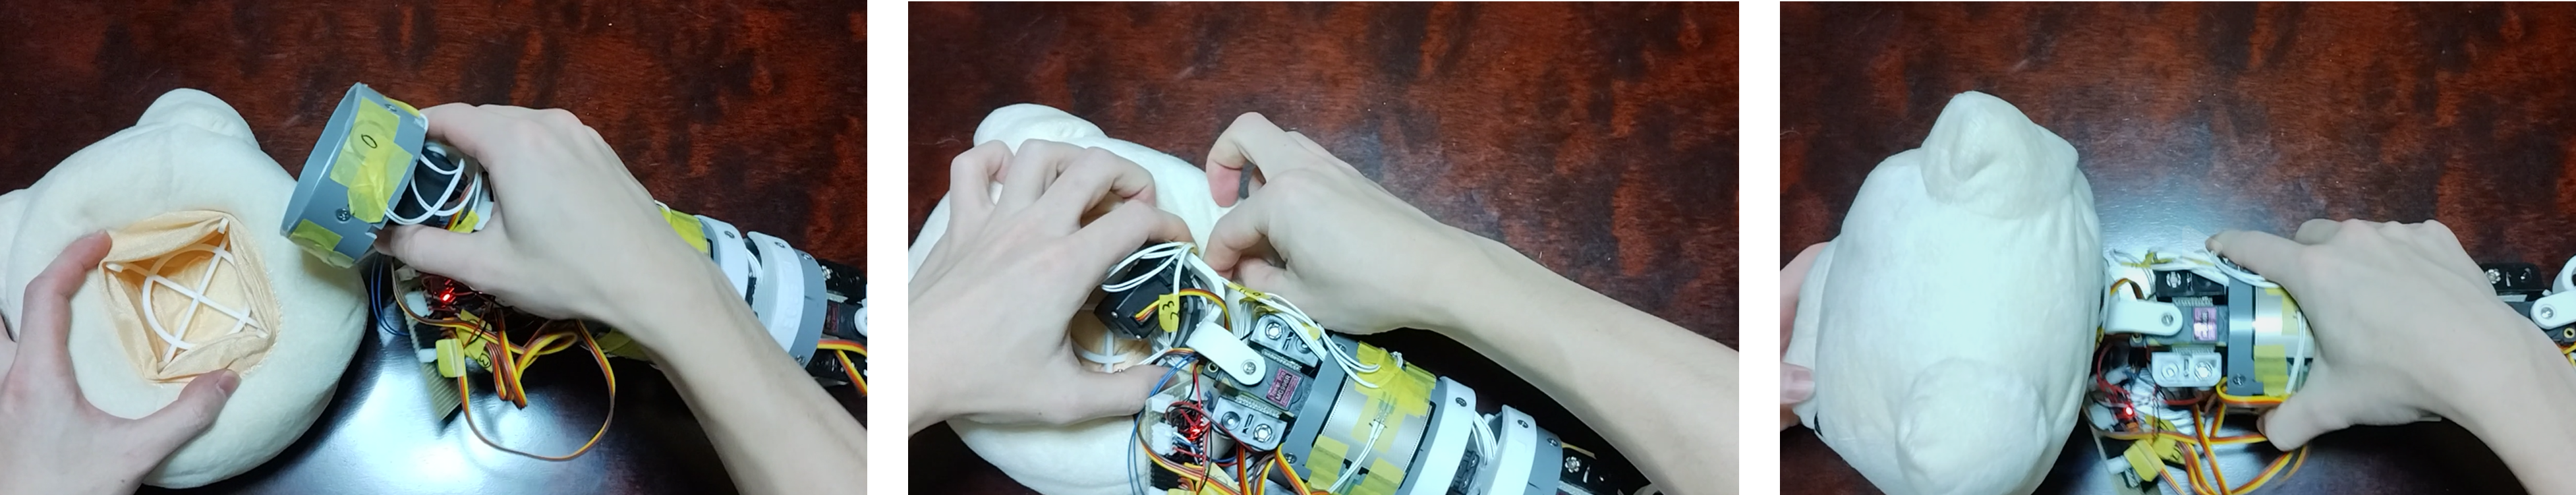
\includegraphics[keepaspectratio,width=12cm,clip]{images/mohutics/embed_dog_head.png}
    \subcaption{頭の取り付け}
  \end{minipage} \\
  \begin{minipage}[c]{\linewidth}
    \centering
    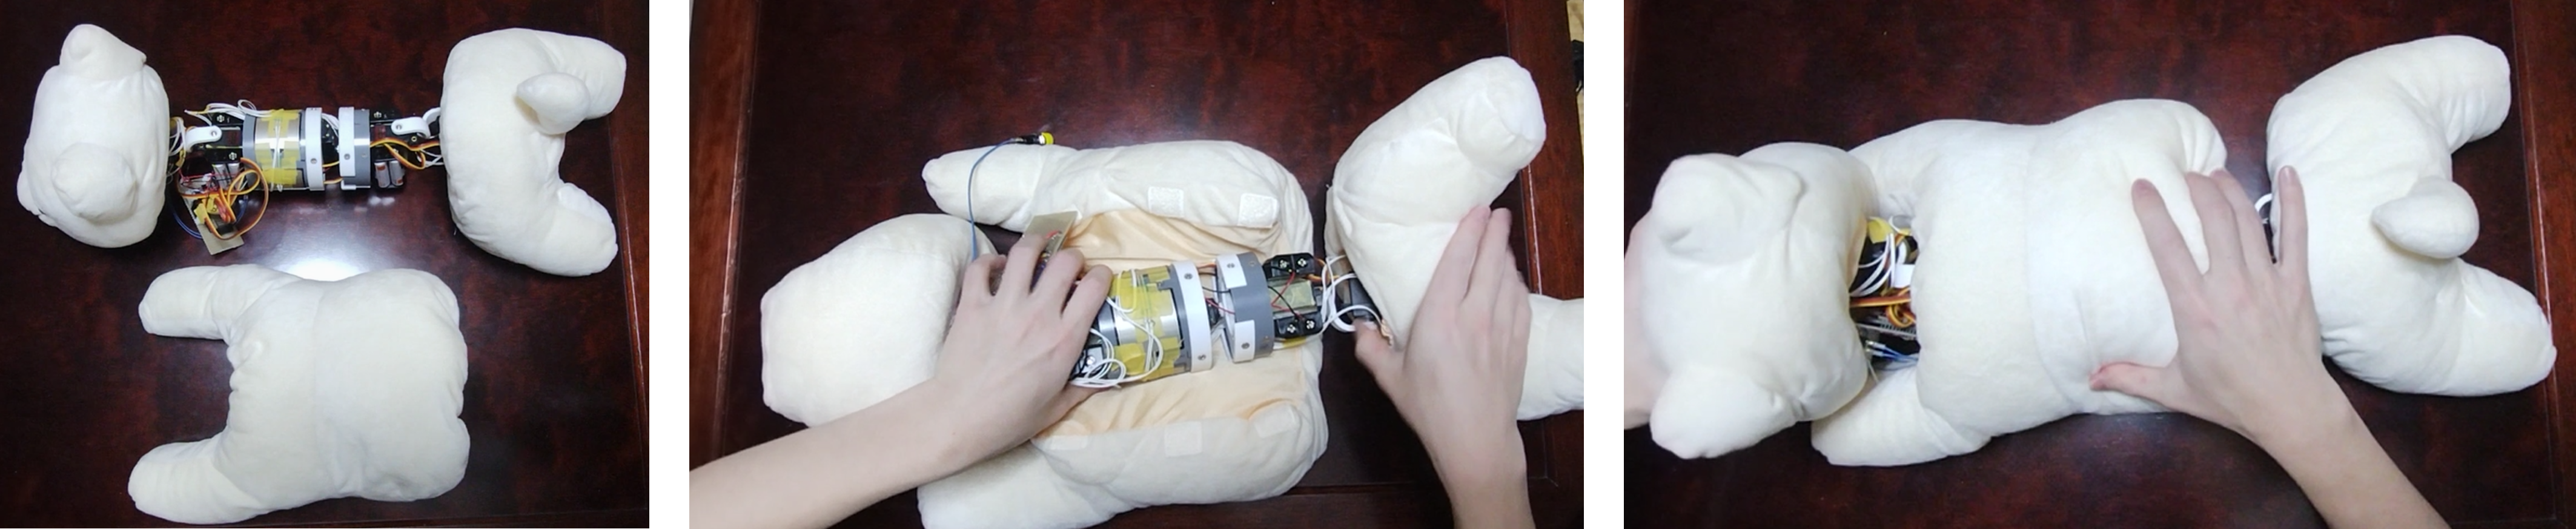
\includegraphics[keepaspectratio,width=12cm,clip]{images/mohutics/embed_dog_body.png}
    \subcaption{胴の取り付け}
  \end{minipage}
  \caption{犬型のぬいぐるみロボットの組み立て}
  \label{fig:mohutics:embed_dog}
\end{figure}

\begin{figure}[htbp]
  \centering
  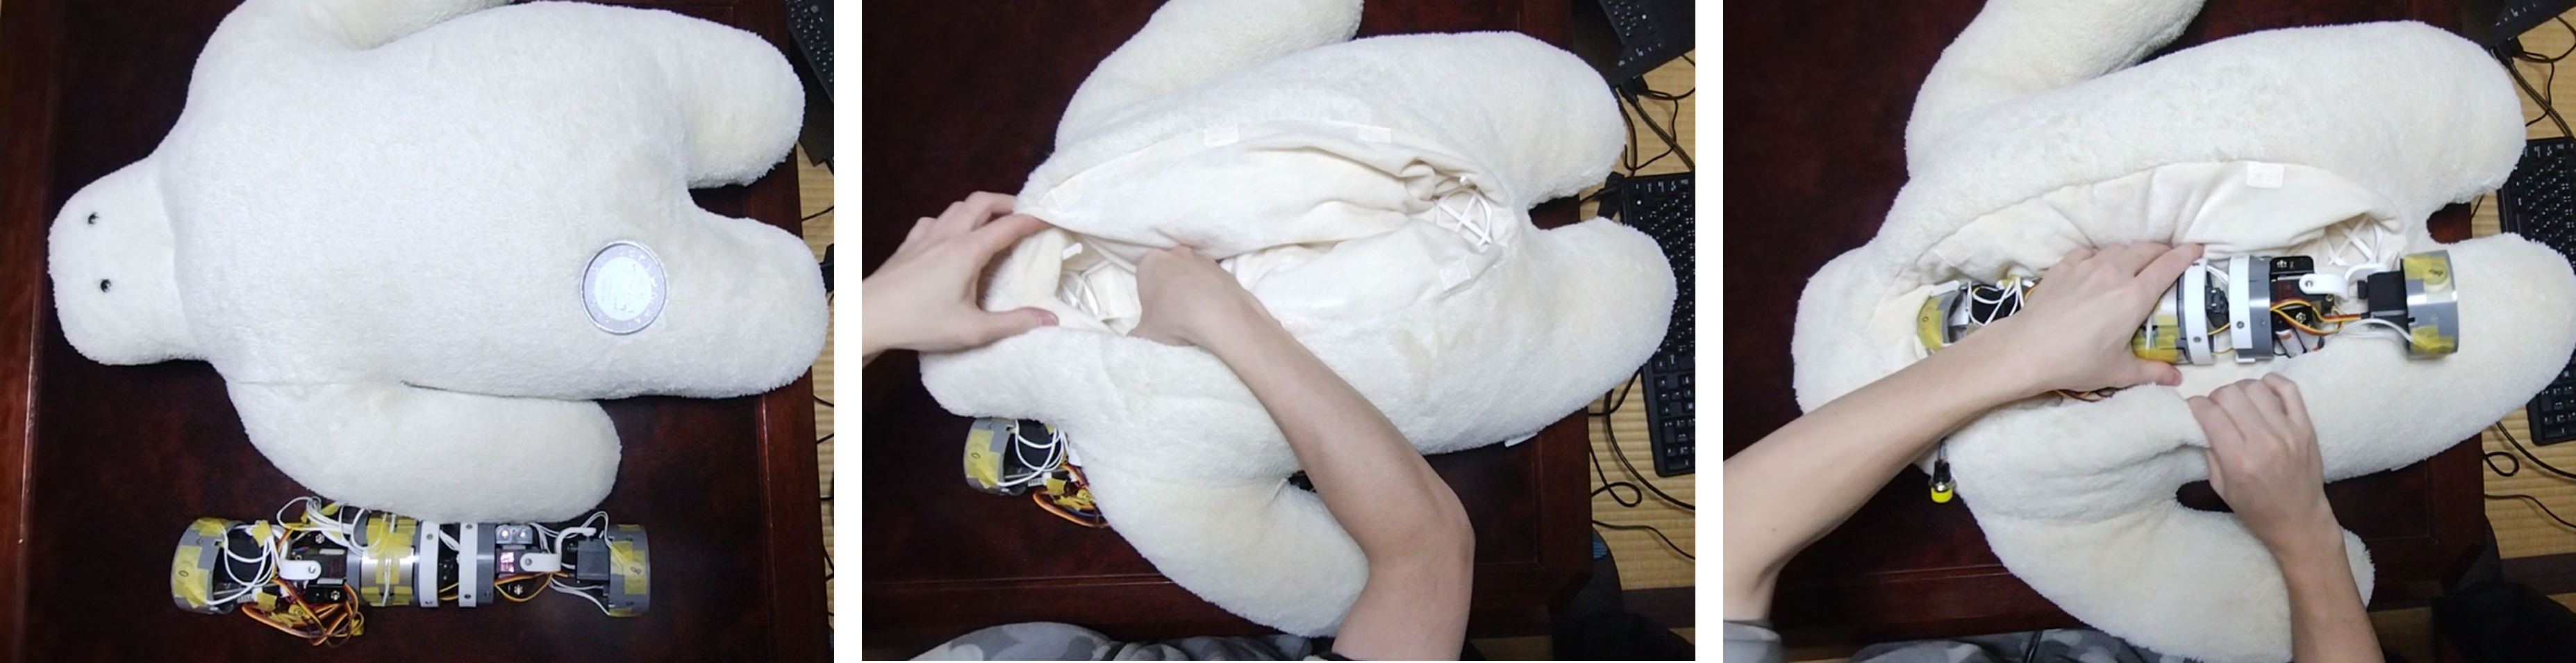
\includegraphics[width=12cm]{images/mohutics/embed_funio.png}
  \caption{人型のぬいぐるみロボットの組み立て}
  \label{fig:mohutics:embed_funio}
\end{figure}

\subsection{ソフトウェア}
ロボットに書き込むソフトウェアの作成にあたり、ぬいぐるみロボットの骨格は共通化されているため、ぬいぐるみの種類によらないハードウェアに近いプログラムとぬいぐるみや機能ごとに異なるプログラムはソースコードを分割し作業の効率化を図った。
ハードウェアに近い部分のプログラムとしては姿勢センサ等のライブラリの実装や感圧センサで使用したPICマイコンのソースコードなどを含む。
さらに、ロボットの機能としては、ユーザがロボットに触れたときに、その外力に抗うように動いて応答する機能などを盛り込んでいる。

また、ぬいぐるみロボットを外部のPCと接続することで、ぬいぐるみロボットに対する人のインタラクション傾向の分析も行った(\figref{fig:mohutics:interaction})。
この分析では、ぬいぐるみロボットに埋め込まれたセンサの情報をPCに送信し、人がぬいぐるみロボットに対してどのようなインタラクションを行うのか測定した。
結果としてはぬいぐるみの種類ごとに形状や容姿から持ち方や触り方などの傾向に差が生まれ、PyTorchによる深層学習と組み合わせることで、センサの値のみからユーザが用意されたぬいぐるみのうちどの種類のぬいぐるみを抱いているかを分類できるようになった。
本検証は試験的なものであるが、今後改良を加えることで、ぬいぐるみロボットが抱き方の傾向から持ち主のみに特定の応答を示すなどの機能が実装できると期待される。

% \begin{figure}[htbp]
%   \centering
%   \includegraphics[width=8cm]{images/mohutics/learning.png}
%   \caption{外部PCを利用したぬいぐるみロボットに対する人のインタラクション方法の分類}
%   \label{fig:learning}
% \end{figure}

% \begin{figure}[htbp]
%   \centering
%   \begin{minipage}[c]{0.96\linewidth}
%     \centering
%     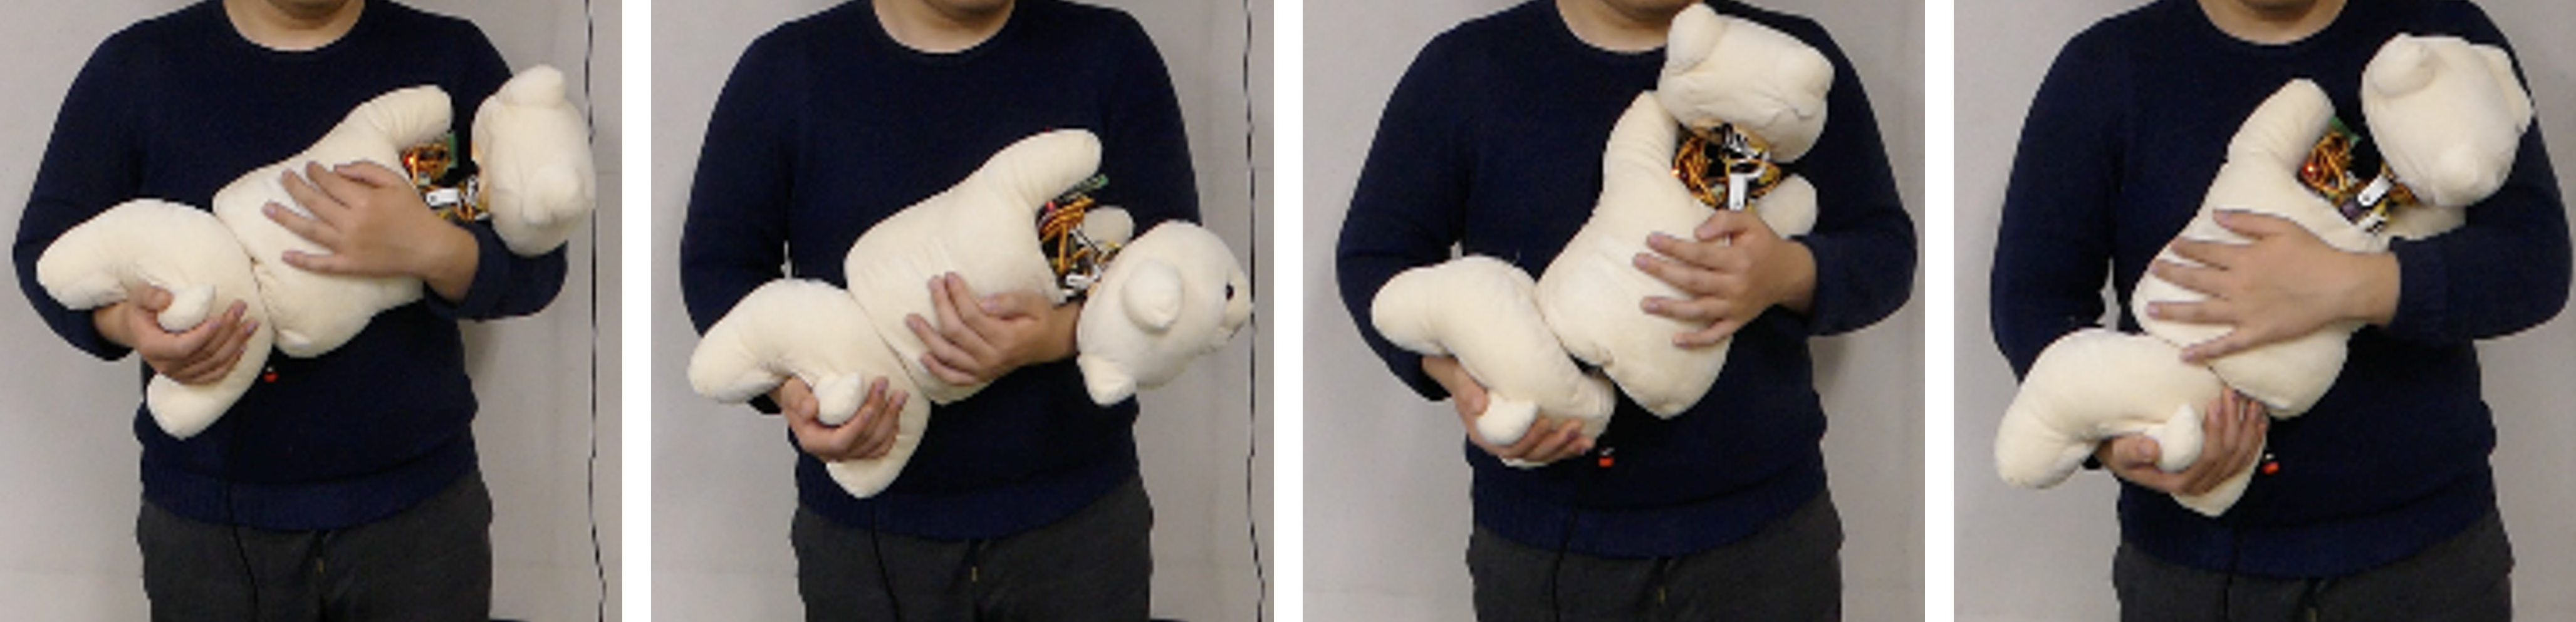
\includegraphics[keepaspectratio,width=12cm,clip]{images/mohutics/dog_interaction_01.png}
%     \subcaption{犬型のぬいぐるみ}
%   \end{minipage} \\
%   \begin{minipage}[c]{0.96\linewidth}
%     \centering
%     \includegraphics[keepaspectratio,width=4cm,clip]{images/mohutics/funio_interaction_01.png}
%     \subcaption{人型のぬいぐるみ}
%   \end{minipage}
%   \caption{人とぬいぐるみロボットのインタラクション傾向の分析の様子}
%   \label{fig:mohutics:interaction}
% \end{figure}
\begin{figure}[htbp]
  \centering
  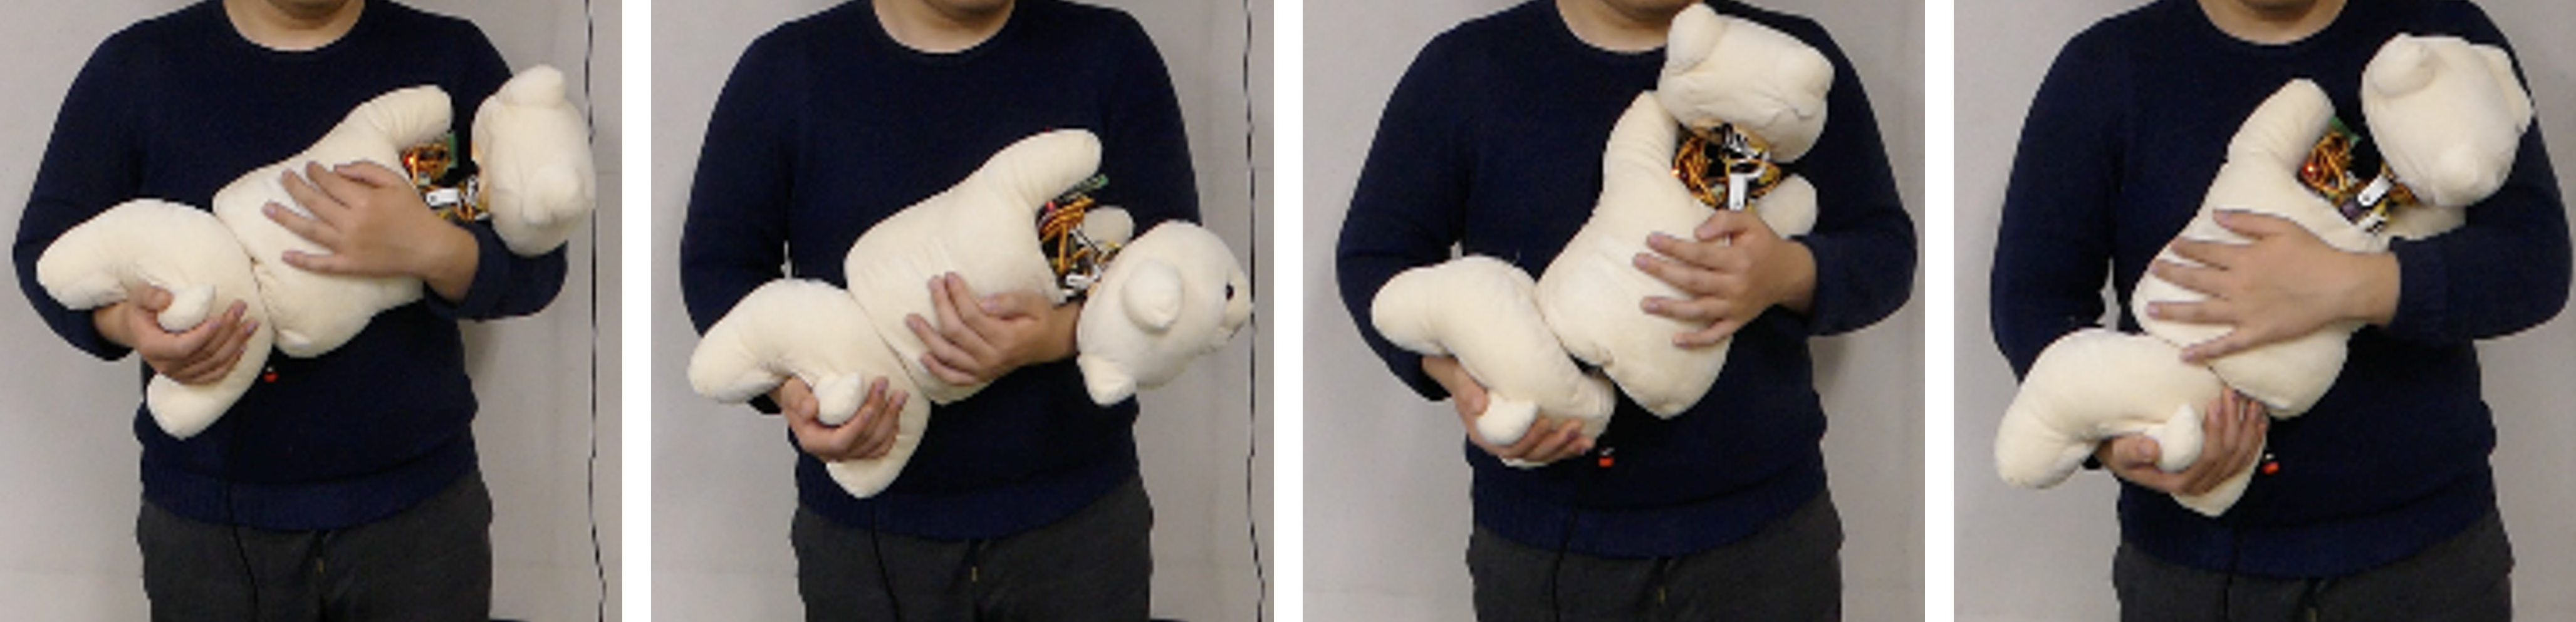
\includegraphics[width=12cm]{images/mohutics/dog_interaction_01.png}
  \caption{人と犬型のぬいぐるみロボットとのインタラクション傾向の分析の様子}
  \label{fig:mohutics:interaction}
\end{figure}


\section{従来の技術との相違}
本システムが従来の愛玩用ロボットと異なる点として、ユーザが簡単に自分の好きな見た目のぬいぐるみロボットを簡単に組み立てられる点が挙げられる。
従来の愛玩用ロボットでは製品ごとにロボットの姿が定まっており、ユーザが自分の気に入った姿のロボットを選ぶことは難しかった。
本システムによって、今までロボットメーカーが愛玩対象のあらゆる機能や仕様を規定し管理していた段階から、ユーザが主体となって自分の好みに寄り添った愛玩用ロボットを迎えられる状況に近づいたといえる。

また、ぬいぐるみと人とのインタラクションに注目し、それを制御に利用した点も重要である。
例えば、ペットではしばしば動物が能動的に人に働きかける。
一方で、本システムのぬいぐるみロボットでは人が自ら触れ合うことで初めてぬいぐるみロボットに刺激や情報を与えられ、それにロボットが応答してコミュニケーションが始まるという流れが実現できる。
ペットもぬいぐるみロボットもともに愛玩対象であるが、その立ち位置には差異があり、ぬいぐるみと人という独特の距離感を活かした本システムはコミュニケーション形式の一つとしても価値があるといえる。

\section{期待される効果}
本システムによって、今まで手軽な愛玩対象を探していた人やぬいぐるみにさらなる愛着を求める人が、ぬいぐるみロボットという形で自分の好みに合う愛玩用ロボットを容易に入手し、癒やし得ることが可能となる。
例えば、子どもが誕生日などの大きなイベントで骨格を買ってもらい、旅先の動物園や水族館などで対応するぬいぐるみを土産に買ってもらうなどすれば、そのぬいぐるみロボットは旅の想い出も相まって唯一無二の存在となるだろう。
さらに、ぬいぐるみロボットが人と触れ合いやすい点を活かして、将来的には本システムを仮想空間に自身のペットとして持ち込んだり、ぬいぐるみを介して遠方の相手とインタラクションを行ったりするなどの利用が考えられる。

このように、本システムは日常に溶け込むロボットとしていち早く人々の生活空間に普及し、社会のロボットへの関心を高めることにも貢献すると期待される。

\section{普及・活用の見通し}
%\section{活用の見通し}
% テンプレートでは「普及(または活用)の見通し」になっていますが、どちらか、あるいは両方を選んで記述をして、見出しをそれに合わせてください。
% 目安です。
% 「普及の見通し」→ユーザ獲得が先にある場合
% 「活用の見通し」→秘匿性が高く自分自身で活用(例えば起業)することが先にある場合
% 「普及・活用の見通し」→両方

本システムを普及させるために、将来的なロボットの設計図及びソースコードのオープンソース化を検討している。
より多くのユーザが手に取り、様々なユーザが自らソースコードを修正し自分の求める機能を追加できる余地を残すことが、ぬいぐるみロボットという発展途上の分野を育む上で重要だと考えるからである。
また、第三者による保守の可能なオープンソースとすることで、ユーザがぬいぐるみロボットという長期にわたって愛されうる存在を安心して迎えられることにもつながる。

さらに、本システムの特長として、ロボットとぬいぐるみという全く異なるノウハウが必要な開発を分割して行える点がある。
したがって、様々なぬいぐるみメーカーに本システムに対応するぬいぐるみの製造を委託し、その際に本システム対応を謳うためのライセンス料を徴収し、その資金をロボットの骨格の開発費の一部に充てるというサイクルを構築できれば、ぬいぐるみの種類を増やしながら本システムを持続的に開発できると考えている。


\section{クリエータ名(所属)}
\begin{itemize}
  \item 小山 高(東京大学 大学院情報理工学系研究科)
\end{itemize}

\section*{(参考)関連URL} % もしあれば
% 関連URLは参考文献のリンクではなくプロジェクト・プロダクトに直接関係するものへのリンクです。成果詳細では参考文献を貼るのはなしです。
\begin{itemize}
  \item X(プロジェクトの進捗を随時掲載予定):\url{https://twitter.com/mohutics}
  \item GitHub(ソースコード公開時に利用予定):\url{https://github.com/mohutics}
\end{itemize}

\end{document}
